\documentclass[12pt]{article}
\usepackage[margin=30mm]{geometry}
\usepackage[comma]{natbib}
\usepackage{todonotes}
\usepackage[toc,page]{appendix}
\usepackage{pdfpages}
\usepackage{graphicx}
\usepackage{url}

\usepackage{listings}
\usepackage{color}
\definecolor{dkgreen}{rgb}{0,0.6,0}
\definecolor{gray}{rgb}{0.5,0.5,0.5}
\definecolor{mauve}{rgb}{0.58,0,0.82}

\lstset{frame=tb,
  language=Python,
  aboveskip=3mm,
  belowskip=3mm,
  showstringspaces=false,
  columns=flexible,
  basicstyle={\small\ttfamily},
  numbers=none,
  numberstyle=\tiny\color{gray},
  keywordstyle=\color{blue},
  commentstyle=\color{dkgreen},
  stringstyle=\color{mauve},
  breaklines=true,
  breakatwhitespace=true,
  tabsize=3
}

\bibliographystyle{agsm}

\begin{document}
\title{Using Facial Recognition to gather Social Media Intelligence}
\author{Jack Neilson}
\maketitle
\newpage
\tableofcontents
\newpage

\section{Literature Review}
\subsection{Background}
\subsubsection{SOCMINT}
Social media intelligence (SOCMINT) is an emergent field in intelligence gathering where data is gathered from social media profiles. Massive amounts of data are added to social media services every day \citep{socmintoverview}, much of it personal, making social media sites a potentially valuable resource when gathering information about groups or individuals \citep{gchqmasssurveillance}. Social networks have also been used as a means of communication between persons of interest to the security services, making mining intelligence from their profiles a high priority \citep{socmintoverview}\citep{policesocmint}.

After the 2011 riots in London that were organised in large part on social media, Her Majesty's Inspectorate of Constabulary stated that the police services were "insufficiently equipped" to effectively use SOCMINT in their response \citep{socmintpublicsafety} which suggests that social media intelligence sources may be woefully underutilised \citep{socmintoverview}. This is not to say that the value of SOCMINT is not realised however, as many intelligence agencies are investing in tools to effectively gather and analyse SOCMINT \citep{socmintpublicsafety} or are performing case studies in to potential uses \citep{bostonbombingcasestudy}.

While traditional human intelligence (HUMINT) focuses on building rapport and a foundation of trust in order to extract information from people of interest \citep{humintinterrogators}, users of social networking websites are much more likely to divulge personal information due to a misplaced senes of privacy \citep{socialmediacontent}. This makes SOCMINT attractive when attempting to gather data with little investment. The amount of data available to gather is vast in comparison to HUMINT sources \citep{socmintoverview}, making mass collection and analysis viable \citep{prismslides}. The nature of SOCMINT makes it easier to analyse than HUMINT, which relies on "tells" and small social cues \citep{humintinterrogators}.

\subsubsection{Uses of SOCMINT}
As previously stated, SOCMINT has seen some emergent use particularly in the security services. The Greek Ministry of Defence has developed a framework to identify individuals fitting certain psychiatric profiles from their social media accounts to allow for early identification of potential insider threats \citep{behaviourdetection}. By identifying factors that multiple intelligence agencies agree make a person more likely to pose an insider threat or negatively influence society (See appendix \ref{appendix:threatgraph}), they were able to map usage habits (intensity, content, popularity) to these factors to draw conclusions about clusters of users. So far, the research has been helpful in insider threat prevention, delinquent behaviour prediction and forensic analysis support.

\subsubsection{Facial Recognition}
Facial recognition is a much more mature area of research than SOCMINT with many examples of industry usage. Facebook uses facial recognition to automate "tagging" photos with the identity of the persons pictured \citep{facebookfacialrecog}, and large companies are now releasing datasets such as YouTube Faces \citep{faceregiondescriptors} in an effort to advance the field.

This is not to say that facial recognition is not without controversy however, as many privacy advocates have pointed out that accurate face regonition could infringe on their right to privacy \citep{gchqmasssurveillance}. David Wood and Lucas Introne have posed that accurate facial recognition could lead to increased levels of surveillance, with no way to "opt out" \citep{facialrecogpolitics}\citep{facialrecogsecurityvsprivacy}.

\subsubsection{Uses of Facial Recognition}
Facial recognition has many practical applications that are already being realised. As noted previously, Facebook uses facial recognition when "tagging" photos. This is presumably done to allow advertisers to more effectively target individual users - for example, a person identified in a photo with a barbeque may receive adverts for propane gas.

Facial recognition is also enjoying a heavy amount of attention from the security services due to it's use in identifying persons of interest. Case studies have been performed using images released to the public to ascertain how effective facial recognition is when looking for a specific person. In particular, Joshua Klontz and Anil Jain performed a case study using the images of the "Boston Bombers" against a set of test data \citep{bostonbombingcasestudy}. Their approach was successful in recognising one of the perpetrators from a picture taken from his social media account (See appendix \ref{appendix:bostonbomber}).

\subsubsection{Constrained vs Unconstrained}
While facial recognition software has come a long way, achieving accuracy rates of up to 99\% on small, consistent data sets \citep{facialrecogidentifyingpoi}, it is still in it's infancy when it comes to identifying people in "unconstrained" images. Images taken in the wild may have large variations in pose, facial occlusion and ambient lighting. This makes it difficult to identify facial features or markers (such as iris distinace, nasal distance, blemishes) which in turn has a negative impact on accuracy rates \citep{unconstrainedfacialrecogbenchmark}. When looking at applications of face recognition software with unconstrained datasets, matches are typically achieved when the test image has similar pose, facial occlusion and lighting as the sample image (See appendix \ref{appendix:bostonbomber}).

\subsection{Prior Knowledge Attacks}
\subsubsection{Social Engineering}
Social engineering in the context of information security refers to the ability of a person to gain access to information or control systems through a user or administrator, rather than through any technical oversight \citep{socialengineeringvulnerabilites}. It is a popular technique against "hardened" targets as technical prevention measures have proven to be ineffective \citep{advancedsocialengineering} making the human users and administrators the weakest link in the proverbial chain. In addition, it is difficult to train users in defenses against social engineering attacks. People believe they would not fall for such a trick despite research showing that humans perform poorly when attempting to detect deception \citep{advancedsocialengineering}\citep{socialengineeringvulnerabilites}. 

Social engineering using e-mail as a medium is ubiquitous \citep{socialengineeringvulnerabilites}. As a generel strategy, the person wishing to gather information will send one or more people an e-mail in hopes of a response (whether that be in the form of visiting a website, replying with their username or password, opening a file etc). Recent studies in realistic environments have had success rates of up to 23\% \citep{socialengineeringvulnerabilites} - this is especially worrying given that even 1 repsondant could compromise an entire company.

Examples of social engineering are not hard to find. In his book \textit{The Art of Deception} Kevin Mitnick describes a young Stanley Rifkin using social engineering to make the biggest bank heist of all time, stealing over 10,000,000 USD \citep{mitnick}. Social engineering attacks are certainly not difficult to perform - recently, a 13 your old child used social engineering to breach the private e-mail of the then-chief of the CIA, John Brennen \citep{cia13yearold}

\subsubsection{Spearphishing}
Spearphish attacks are a subsection of social engineering attacks wherein an attacker sends a malicous e-mail to a user that has been crafted using information that would make it seem authentic \citep{spearphishing}. For example, a normal social engineering attack using e-mail might send boilerplate messages to all personnel in a department to attempt to gain access to a network account. By contrast, a spearphish attack may use the names of specific people in the department, the location of the department, a spoofed e-mail header to make it seem as if the message came from within the department, and so on.

Social engineering attacks have proven to be effective at accessing sensitive information even when significant effort has been expended to secure it. A recent spearphishing campaign was conducted against 500 US military cadets - over 80\% clicked the link in the e-mail \citep{spearphishing}. Spearphish attacks are even more effective than "blind" phishing because of the additional information included in the e-mail which lulls the user in to a false sense of security (particularly when the information could be wrongfully considered "sensitive", for example including a manager's name and phone number).

Spearphish attacks in particular are difficult to mitigate against. They target the human element in information security making technological defenses insufficient \citep{spearphishing}. Education on spearphishing is not adequate to mitigate the potential threat either, as shown by William Pelgrin's exercise. He sent 10,000 New York State employees a phishing e-mail, and had a success rate of 15\% (that is, 15\% of users clicked the link in the e-mail then attempted to enter their passwords). The experiment was repeated after four months, with some success shown as the experiment had a success rate of 8\% \citep{spearphishingresults}. It must be remembered however that even a single successful spearphish attack could lead to a breach of information security.

\subsection{Intelligence Gathering}
\subsubsection{SOCMINT}
Social media intelligence (SOCMINT) refers to information gathered from social media profiles hosted on social networks. It is an emergent field in open-source intelligence (OSINT), which relies on gathering information users divulge about themselves in the public domain. It is characterised by the massive amount of data available \citep{socmintoverview} and the difficulty of analysis \citep{socmintlitreview}. An overview of subjects relating to social media intelligence gathering follows below.

\subsubsection{HUMINT}
Human intelligence (HUMINT) pertains to the gathering of intelligence from individual human subjects. Information may be divulged non-consensually e.g. in the case of interrogation \citep{criminalvshumint}, or consensually in the case of clandestine information gathering \citep{clandestinehumint}. 

Non-consensual information gathering via interview or interrogation has only recently become a subject of study for the general public \citep{humintinterrogators}. 

Consensual information gathering sits in a much more grey area. Presenting yourself as somebody else may not be illegal depending on the circumstances, however it poses several moral questions. Clandestine intelligence gathering is still an extremely effective strategy, particularly when attempting to gather sensitive information which may be more heavily protected e.g. airgapped, firewalled \citep{clandestinehumint}. This makes it attractive during wartime or times of civil unrest \citep{humintni}\citep{humintcyberage}

Using a human intelligence approaches when gathering information has several downsides. It is a high risk strategy, as should a person be found out the consequences can be severe \citep{humintni}. The potential reward of sensitive information may be deemed to not be worth the risk. It goes without saying that HUMINT does not scale particularly well - it is a useful tool when attempting to extract information from a single person or small group, but it is much less useful when gathering information about larger groups. It relies on trust being built and may be ineffective when attempting to gather information from targets trained in tradecraft \citep{humintni}\citep{clandestinehumint}\citep{humintcyberage}.

\subsubsection{Individual vs Group Data}
Much of the research done on social media intelligence has focused on group trends or finding subsets of a population \citep{socmintpublicsafety}\citep{socmintoverview}. Comparatively, fairly little research has been done on identifying a single person of interest from a social network service.

A practical example of where SOCMINT has been used in the real world is the framework created by Kandias and Stavrou, in which features of a social media profile such as number of friends, "friend hops" standard deviation, psychiatric profiling and usage intensity are used to predict groups of interest that may become radicalised \citep{behaviourdetection}. While this is certainly very useful, it focuses more on identifying groups by some common factor rather than identifying a single person of interest for further analysis.

\subsubsection{Quantity of Information}
Having limited information is not a problem when gathering social media intelligence. Rather, the opposite is true - 250,000,000 photos are added to Facebook every day \citep{socmintoverview}. The vast amount of data is what makes searching for social media so difficult (and nigh on impossible in real time).

While the total amount of data added to social networking websites is extremely large, the information about a single user may be fairly small especially if the user has been trained to release as little information as possible \citep{behaviourdetection}. This may make targeting single persons of interest less valuable, however should information "leakage" occur the potential payoff is high. It should be remembered that scanning social media profiles incurs little to no risk, something that cannot be said of human intelligence.

\subsubsection{Accessibility of Data}
As discussed previously the amount of data pushed to social networking websites is massive. This does not mean that all social networking data is readily accessible. Users may set privacy settings to disallow unauthorised parties from viewing their profile, or particular parts of it. This can be mitigated by having the service allow access, however acquiring access as a party of one may prove difficult.

Several social networking services also impose rate limits on their interfaces (for example, Facebook imposes a limit of 100 API calls per user of an application as well as limits on CPU time used). These limits obviously make searching through the entire data set of profiles unfeasible without allowances made on the side of the social network. 

\subsubsection{Uses}
Usage of social media intelligence has been limited in large part due to the difficulty in analysing such large amounts of data for small snippets of useful information \citep{socmintoverview}. There are, however, some interesting case studies available.

In April 2013, Edward Snowden leaked a deck of slides used by the NSA to brief people on the "PRISM" program \citep{prismslides}. These slides detailed how the NSA uses mass surveillance with cooperation from companies including Google, Facebook, and Apple, to conduct surveillance against persons of interest. As a government agency enabled by the oversight committee, the NSA has the power to require large social networking services like the ones listed to allow them access to their data.

As mentioned previously, Kandias and Stavrou have developed a framework for using social media intelligence for predicting and mitigating insider threats while working at the Information Security and Critical Infrastructure Protection Lab at the University of Athens \citep{behaviourdetection}. The framework focuses on analysing the psychology of the subjects using their social media posting habits. It shows that seemingly inconsequential data such as posting frequency may still be useful when analysing social media intelligence. An example graph to find the amount of "klout" a social media user may have in the Nereus framework is referenced in Appendix \ref{appendix:connectiongraph}.

\subsubsection{Challenges and Constraints}
There are several challenges to consider when collecting and analysing data for social networking services. First is the issue of privacy. Many people see social media profiles in a similar setting as a meeting between friends, and as such post things which they perhaps would not say or show in public \citep{socialmediacontent}. The chilling effect of public scrutiny, or even direct surveillance, does not seem to put a damper on this.

There are some that feel that police surveillance of social networks is too pervasive \citep{socmintlawenforcement}, and encroaches on their right to privacy. Despite the effectiveness of social media intelligence gathering, it may be harmful to law enforcement's public image if it continues to utilise SOCMINT.

As far as the law is concerned, information posted on social networking sites is considered to be in the public domain. This makes it legal for law enforcement to gather social media intelligence, provided they do it the same way an unprivileged user would. Several social networks have clauses against mass data collection in their Terms of Service, however it is theorised that this is to prevent competition from other companies when selling said information to advertisers.

\subsection{Facial Recognition}
\subsubsection{Current Applications}
Police and military uptake of face recognition technology is widespread. For instance, police in the United Kingdom recently used cameras to scan people's faces at the "Download" music festival \citep{policefacerecog}. These images were then compared with a database of custody images across Europe, to identify known criminals for the purposes of crime prevention and outstanding warrant execution.

Facebook also uses face recognition on photos uploaded to its service \citep{facebookfacerecog}. By comparing face mappings to the known face mappings of yourself and immediate friends, it can suggest "tags" of who is in the image which presumably makes the information contained within the image more valuable to advertisers.

\subsubsection{Unconstrained Facial Recognition}
Unconstraned facial recognition is a subset of facial recognition which focuses on identifying faces in images with variations in pose, lighting, and facial occlusion. It is significantly more difficult than facial recongition which imposes constraints on these conditions.

Unconstrained facial recognition is typically used in situations where a subject is unaware or unwilling. As already mentioned, it was used in a case study by Klontz and Jain where they compared the images released by the FBI of Tamerlan and Dzhokhar Tsarnaev (the "Boston Bombers"). They found that by comparing the released images taken from security cameras to images on social media in an unconstrained setting, they could positively identify one of the brothers \citep{bostonbombingcasestudy} (see Appendix \ref{appendix:bostonbomber}).

\subsection{Existing Solutions}
\subsubsection{pipl}
\url{pipl.com} is a popular web service that allows users to search a database of people by name, e-mail, social media username, phone number, or location. It is aimed at de-anonymising people that use pseudonyms or that do not publicly associate identifying information with their e-mail or social media username by cross-referencing information from several sources. For example, a person may associate their e-mail but not their phone number with a username on a social media service, and then associate the same username with their phone number but not their e-mail address on a different social media service. With this method pipl can effectively collate identifying data about a large sample of people and make it searchable, which is evidently useful for many business applications (particularly within advertisement, as it allows for targeted adverts to be sent to the same person over several social media networks). It's list of clients include large companies within the social media and personal data sectors such as Twitter, equifax and Experian \citep{pipl}.

\subsubsection{192}
\url{192.com} is a similar service to pipl, however it allows for a more advaced search with more terms to restrict or search on. As well as using social media profiles it uses publicly available information (OSINT) such as the electoral register to enhance its data set. It claims to have 750 million records, far less than pipl's over 3 billion (although the records kept by 192 are much more detailed). The main feature of 192 is that it allows users to search for details about entities other than people, such as schools or businesses.

\subsubsection{Facebook}
Facebook itself offers fairly primitive search functionality, allowing users to search for posts, people, photos, videos, pages, places, groups, and events. While this may seem to be fairly extensive, it should be noted that the intended use of the search function is to allow userse to make more connections. The searches users can perform will therefore be tightly restricted - for example, when searching for people the search may only show those people that are indirectly connected through other friends, known connections, or people in close proximity \citep{facebookpeoplesearch}. The Graph API that Facebook exposes allows users to search outside of these restrictions, however as discussed previously it is difficult for a party of one to use the Graph API for large-scale searches due to rate limits and Facebook's privacy settings \citep{facebookgraphapi}. 

Even with these limitations, Facebook is still a very useful service for enumerating identifiable information about a person of interest provided the user has some basic information such as the person of interest's full name.

\subsubsection{Gaps in Functionality}
The services listed above are extremely useful when attempting to gather more information about a person of interest. Given some basic identifying information such as username, given name, e-mail address etc. they can be used to effectively build a profile of searchable person. Where they fall short however is when a person of interest needs to be identified from a collection - the amount of data returned when searching for location or place of residence alone is far too large to sift through. Even Facebook's search falls short when trying to identify a single person from a potentially large collection, as the lack of customisable search restrictions means that the result of a search is unlikely to be able to be processed in a reasonable amount of time.

With the exception of Facebook, the services listed aggregate social media profiles in order to hold as much meaningful information about individuals as is feasible. This necessitates that some information must be omitted when collating from several social media networks. One of the pitfalls of these services is that several of the omitted items can be very useful when restricting searches - for example, a profile picture may prove useful for identification if a user has a reference image of a person of interest.

A potentially large gap in functionality is that lack of "soft" comparisons. The services above perform well when doing direct comparisons, such as having a specific name or a name matching a regular expression. They do not offer search functionality allowing for some margin of error such as a name matching a regular expression or having a Hebbian distance of 1, or having a face harvested from a profile picture be similar to a test image.

\newpage
\section{Methodology}
\subsection{Overview}
The software implemented will be in the form of a Python command line program, which allows users to specify an input image and data set to check it against. Additional identifying information such as name, date of birth etc. should also be utilised if given. The data sets the software references must come from social networking websites (or in the case of this proof of concept, a data set which is an accurate representation).

As its output, the software must show the five most similar faces in the data set to allow for human verification. They should be presented with information that was gained from their social media profiles such as age, gender, name etc., as well as the similarity to the test image. In the case that the software is being ran headlessly, the results should be available in a file format which includes an image of the match and a representation of their social media profile.

\subsection{Functional Requirements}
\subsubsection{Face Recognition}
The software must implement a method of facial recognition, to rank a set of faces by similarity to a given test image. The test face must be extracted from the input image. The top 5 matches should be outputted, along with relevant identifying information.

\subsubsection{Social Media Integration}
The software must have the ability to use social networking websites as it's data set when comparing a test face. It would be desirable for the software to have the capability to use other identifying information alongside the test image to narrow the search space. Due to limited time and resources, test accounts may be used as a proof of concept.

\subsubsection{Headless}
The software should be able to function without a GUI, since the requirement of being able to use extremely large data sets may require deployment to a large server cluster or to a cloud.

\subsubsection{Multithreaded}
Where applicable, the software should make full use of parallelisation to increase its speed and resource utilisation. This is particularly important when working with large data sets.

\subsection{Non-functional Requirements}
\subsubsection{Accuracy}
The software should have a \textit{relatively} high success rate when identifying a person from a social media collection. Note that typical facial reocgnition performance in unconstrained environments achieve a maximum success rate of ~30\%.

\subsubsection{Usefulness}
The information gained by using the software should help when crafting prior-knowledge attacks, increasing their effectiveness.

\subsubsection{Cross-Platform}
The software must be cross-platform to allow for easy deployment to servers or a cloud.

\subsubsection{Imprecision Tolerance}
The software should attempt a best guess when using an input image with less than ideal pose, facial occlusion or lighting. Inferior results when given a test image like this are acceptable to a degree.

\subsubsection{Usability}
The software is being developed for use by information security professionals in the form of a command line tool. This is ubiquitous in the industry, so no more than a cursory glance over the usage information should be needed to begin using the tool.

\subsubsection{Facial Recognition Libraries}
Due to time constrants, reimplementing facial recognition capabilities is not feasible. Therefore, the software should make use of already existing facial recognition libraries, in particular dlib or OpenCV.

\subsubsection{Language}
The software should be written in Python to allow for easy use of face recognition programs and rapid prototyping.

\subsubsection{Time Spent}
The software must be able to complete the above task in the same time or less than a human.

\subsubsection{Documentation}
The software should have at a minimum a man page and usage information. More documentation would be beneficial.

\subsubsection{Testing}
The software will be tested using a comination of publicly available face recognition datasets including Labeled Faces in the Wild, the CMU Face in Action database, and the SCFace database. \todo{Include final list of databases}

\todo{Talk about languages, other choices}

\newpage
\section{Implementation}
\subsection{Face Recognition}
The application has been developed using the face recognition module created by A. Geitgey:

\url{https://github.com/ageitgey/face\_recognition/}.

It is an easy to use facial recognition library build on top of dlib. It exposes a python API, making it ideal for this project. It also boasts an accuracy rate of up to 99.38\% on the LFW data set.

Alternate libraries (such as dlib) that were investigated were found to either have a much higher barrier to entry, or a much lower accuracy.

\subsection{Test Server}
\subsubsection{nginx}
To test the application, nginx is used to serve static content as well as as a reverse proxy. Nginx was chosen over Apache or another native Python webserver due to its capability at handling massive concurrent requests, its flexibility, and its speed at server static content. Since the application makes several connections simultaneusly and requests large amounts of images, nginx was ideal.

\subsubsection{cherrypy}
To serve a dynamic description of where profiles and their respective images are located, a cherrypy server was implemented which expands a glob from the test directory (which contains the test data sets) then returns a json representation of them. As noted earlier, nginx acts as a reverse proxy to this service

\subsection{Portable Module}
The application has been developed in a modular fashion. To this end, a run file has been provided alongside a python module. The python module includes the logic for retrieving profiles from a web service and setting up multiple threads to compare face mappings, whereas the run file comes with some pre-processing and default arguments. Ideally, the module should be re-usable for other web services.

\subsection{Threading}
The application has been developed to make use of multiple threads. The main thread in \textit{facegather.py} controls these threads and their results using locks, thread-safe queues, semaphores, and the thread.join() method.

The producer / consumer consumer model was useful when developing the application. In this context, the producers retrieve profiles from the social networking service and the consumers compare the retrieved profiles to the test data given and store the result.

\subsection{Command Line Interactivity}
Rather than use a graphical user interface (GUI), the application makes use of command line arguments (see Appendix \ref{appendix:commandlineargs}). There are several reasons for this; it cuts down on needless computational cost by eliminating the overhead of a GUI, it allows the OS the application is running on to be "headless" (i.e. run with only a command line or remote connection for user interactivity) again cutting down on overhead, and it allows for easier integration in to scripts (for example, appending logs to a log file using the POSIX >> operator).

One potential issue when using an application without a GUI is presenting the results. The application persists its results in a JSON format for use by other applications or for direct consumption by the end user. \todo{results}

\subsection{Social Network Interactivity}
Since this project has been done on a fairly small scale in a short time frame, it was not possible to gain access to a large social media platform to perform testing (ignoring the obvious ethical issues with such an approach). Instead, the test environment has been set up in such a way as to mirror the way in which a social media API may be presented - with an array of profiles, each one having a link to some related resources.

\subsection{Challenges}
\subsubsection{Loading Images from Memory}
Since the application retrieves images remotely over the internet, it makes sense to manipulate the images directly from memory. This avoids filesystem reads and writes, which are several magnitudes slower than memory reads and writes. The time save is massive, especially when repeated over thousands of images.

Unfortunately the face recognition library does not support loading images from memory, instead providing a method (load\_image\_file(uri)) to load images from the local file system. Upon inspection this method loads an image file from disk in to a Python Imaging Library (PIL) Image object, then casts it to a numpy array to allow for encoding operations. To mirror this method for use with images loaded to memory, the application uses the PIL Image.open() method on the raw response stream from the social network web server to create an Image object, then casts it to a numpy array. This achieves the same result as loading the image from the local file system significantly more efficiently.

\begin{lstlisting}
# Load an image in to memory from local or remote sources
def load_images(uri, remote=True):
    if remote:
        print('Retrieving image from ' + uri)
        resp = requests.get(uri, stream=True)
        resp.raw.decode_content = True
        img = Image.open(resp.raw)
        return fr.face_encodings(numpy.array(img))
    else:
        print('Retrieving image from ' + uri)
        img_array = fr.load_image_file(uri)
    return fr.face_encodings(img_array)
\end{lstlisting}
\textit{Above: A function with an optional keyword parameter to load an image from either a local or remote source.}

\subsubsection{Maximum Loaded Images}
A potential problem when using the producer / consumer model is that producers may produce too much data, filling all available memory and leading to a crash. To solve this a maximum loaded images parameter can be supplied when running the application, which will cap the number of face encodings loaded into memory at that number. This has been implemented using a semaphore initialised with the maximum number of face encodings to be loaded. Each producer thread calls acquire() before loading a set of encodings in to memory, and each consumer thread calls release() when the encoding has been compared and the memory can be freed.

\begin{lstlisting}
# Producer thread
		self.waiting_counter.acquire()
            if profile_queue.empty():
                return
            profile = profile_queue.get()
            
# Consumer thread
            img = img_queue.get()
            ---
            Comparison happens here
            ---
			self.counter.release()
\end{lstlisting}
\textit{Above: The producer thread calls acquire() on the semaphore before loading mappings in to memory, and the consumer thread calls release() on the semaphore after the memory used for mappings has been freed.}

\subsubsection{Multiple Threads for Producing and Consuming}
As it stands, the application has been developed with mulitple threads in mind. The user can define how many threads should be used for downloading images and producing face mappings via the --cthreads argument, and how many threads should be used to compare face mappings via the --pthreads argument. This allows for much higher processor utilisation than a single threaded application, as all CPU cores can be utilised.

While the application processes images orders of magnitude faster than it would had it been single-threaded, it may still be too inefficient for use on particularly large data sets. It is also difficult to scale due to its singleton nature. In the future it may be worth refactoring to make use of a discrete GPU, or to make use of specialised libraries for big data processing such as MapReduce.

\subsubsection{Thread Object Access Control}
To control object access between threads two Queue objects are used. One contains a JSON representation of all of the profiles in the search spaces and is only accessed by the producer threads, and the other is used by producer threads to send face mappings of profiles to consumer threads. These objects are guaranteed to be threadsafe, meaning that both the put() and get() operations are atomic. To control access to the result object that multiple consumer threads may try to access, a Lock() is passed in the consumer constructor. Before a consumer accesses the result object it must first call lock.acquire() which will block if another thread has acquired the lock first. After a consumer has finished writing to the result object it releases the lock by calling lock.release(), allowing other consumer threads access.

\begin{lstlisting}
				self.result_lock.acquire()
                self.result.add([distance, img[1]])
                self.result_lock.release()
\end{lstlisting}
\textit{Above: The result object is not thread-safe, so must have a lock around it.}

\subsubsection{Result Retrieval}
Having a "top 5" result as was initially planned would require many comparison and list traversal operations. It would also make having multiple consumers pointless, as only one thread would be able to do comparisons at a time. Rather than having the top 5 matches, the result returned is now all faces that match the test face within a given threshold (by default, face distance $<$ 0.6).

\subsubsection{Command Line Arguments}
The application can take many command line arguments to customise its use. Having the user fill out and remember every one of these arguments would make the application unintuituve and difficult to use. Therefore, the decision was made to make heavy use of optional keyword arguments both when running the program (e.g. --cthreads=1) and in functions within the application. This allows the user to specify some, all, or none of the optional parameters and still have the application function correctly. 

\begin{lstlisting}
def search(test_face_location,
           uri,
           no_producer_threads=None,
           no_consumer_threads=None,
           max_loaded=None,
           threshold=None,
           name=None):
\end{lstlisting}
\textit{Above: The search function uses several keyword arguments with default arguments, then checks and loads with defaults if not supplied before continuing.}

\subsubsection{Inter-Thread Communication}
The only inter-thread communication required by the application is for the consumer threads to be signalled when there are no more face mappings to compare. To this end, the main thread which spawns both the producer and consumer threads blocks by calling producer.join() on all producer threads. One all producer threads have returned, the main thread pushes a sentinel object on to the end of the face mapping queue. It then blocks by calling consumer.join() on all consumer threads. Once a consumer thread pops the sentinel object, it adds another sentinel to the end of the queue (for further consumer threads to consume) then returns. This guarantees that there is no unconsumed data, and that the consumer threads do not terminate prematurely.

\begin{lstlisting}
	# Main thread
    for processor in processor_list:
        processor.join()
    img_queue.put(sentinels.NOTHING)

    for recogniser in recogniser_list:
        recogniser.join()
        
    # Consumer thread
    if img == sentinels.NOTHING:
        img_queue.put(sentinels.NOTHING)
        return
\end{lstlisting}
\textit{Above: The main thread blocks until all producer threads are finished, then pushes a sentinel object to the end of the queue, then blocks until all consumer threads are finished.}

\section{Testing}
\section{Results}
\section{Evaluation}
\section{Conclusion}

\newpage
\bibliography{citations}

\newpage
\begin{appendices}
\section{Threat Graph}
\label{appendix:threatgraph}
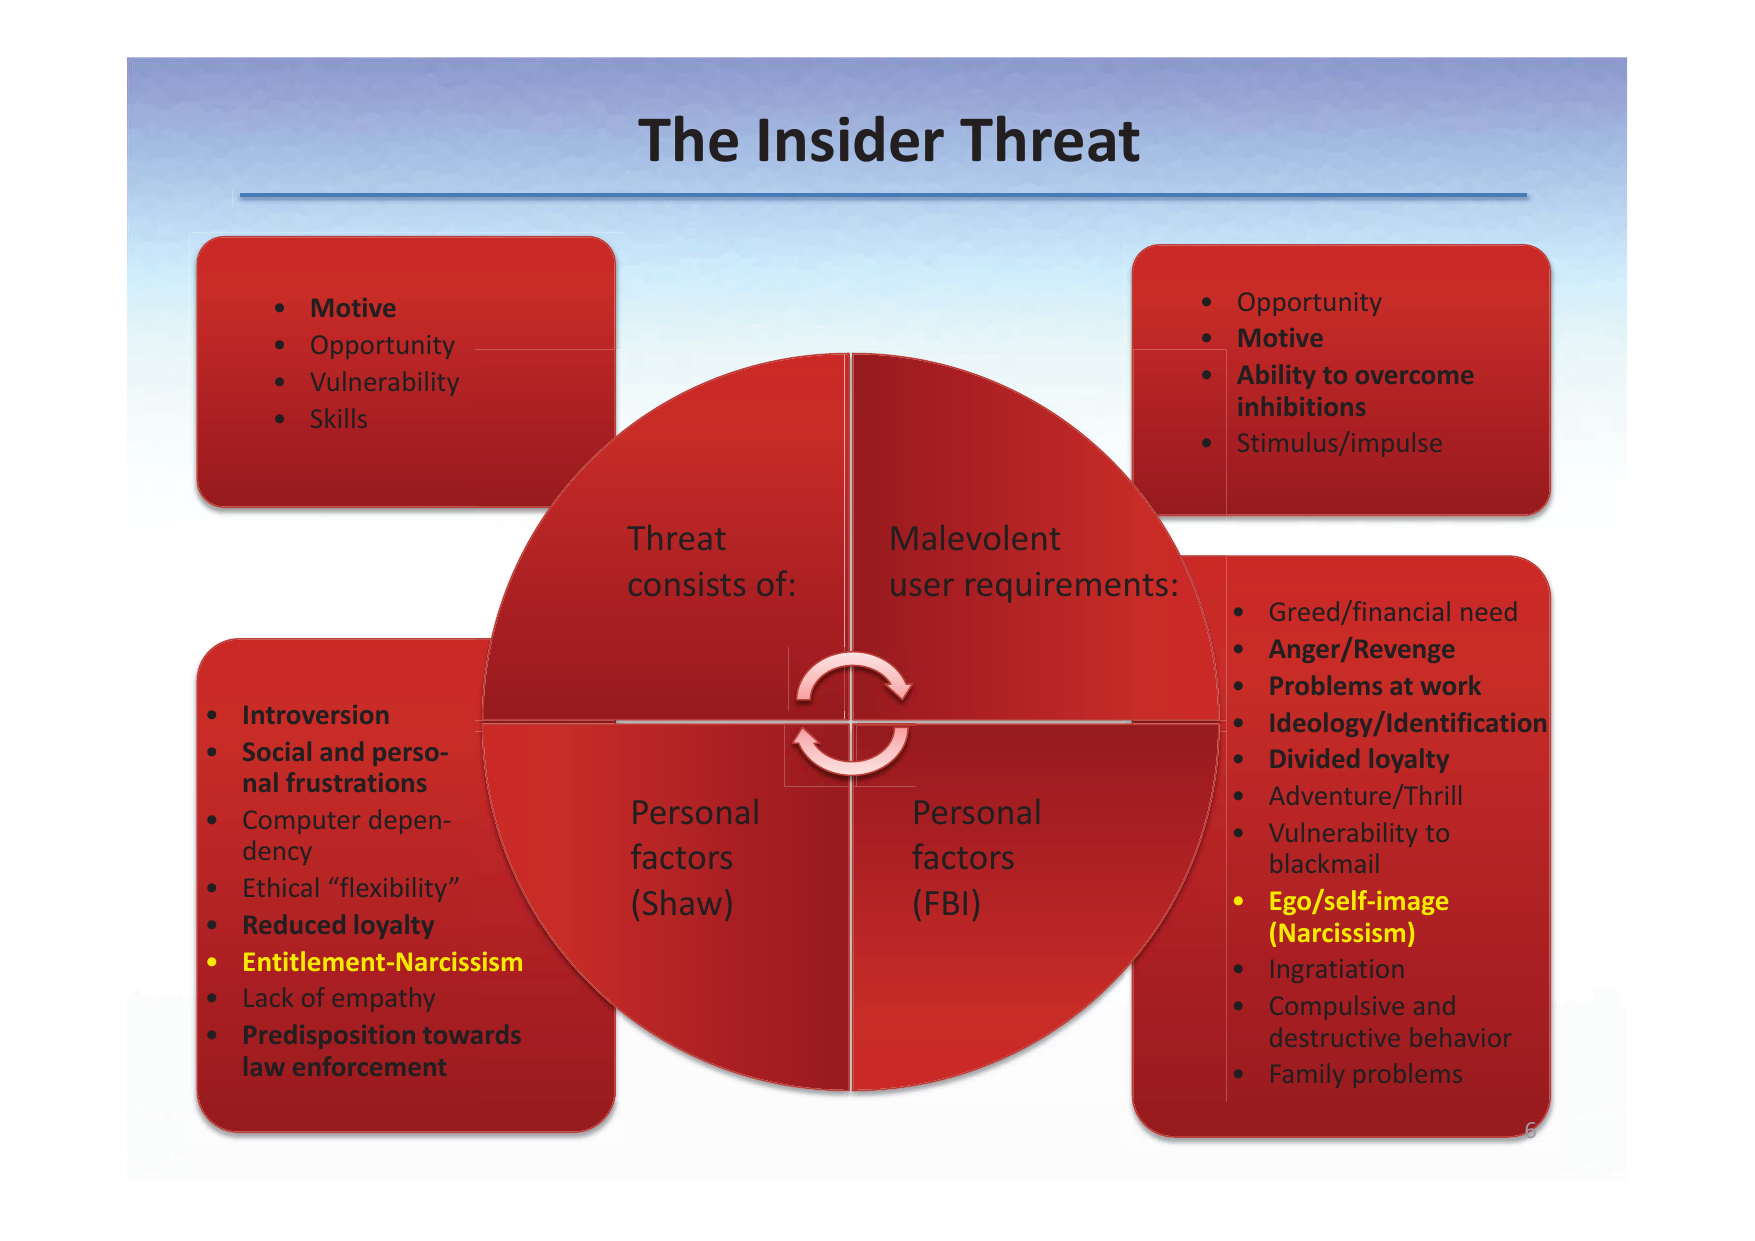
\includegraphics[width=\linewidth]{res/threat_graph.png}
Graph of insider threat factors \citep{behaviourdetection}.

\section{"Boston Bomber" Identification}
\label{appendix:bostonbomber}
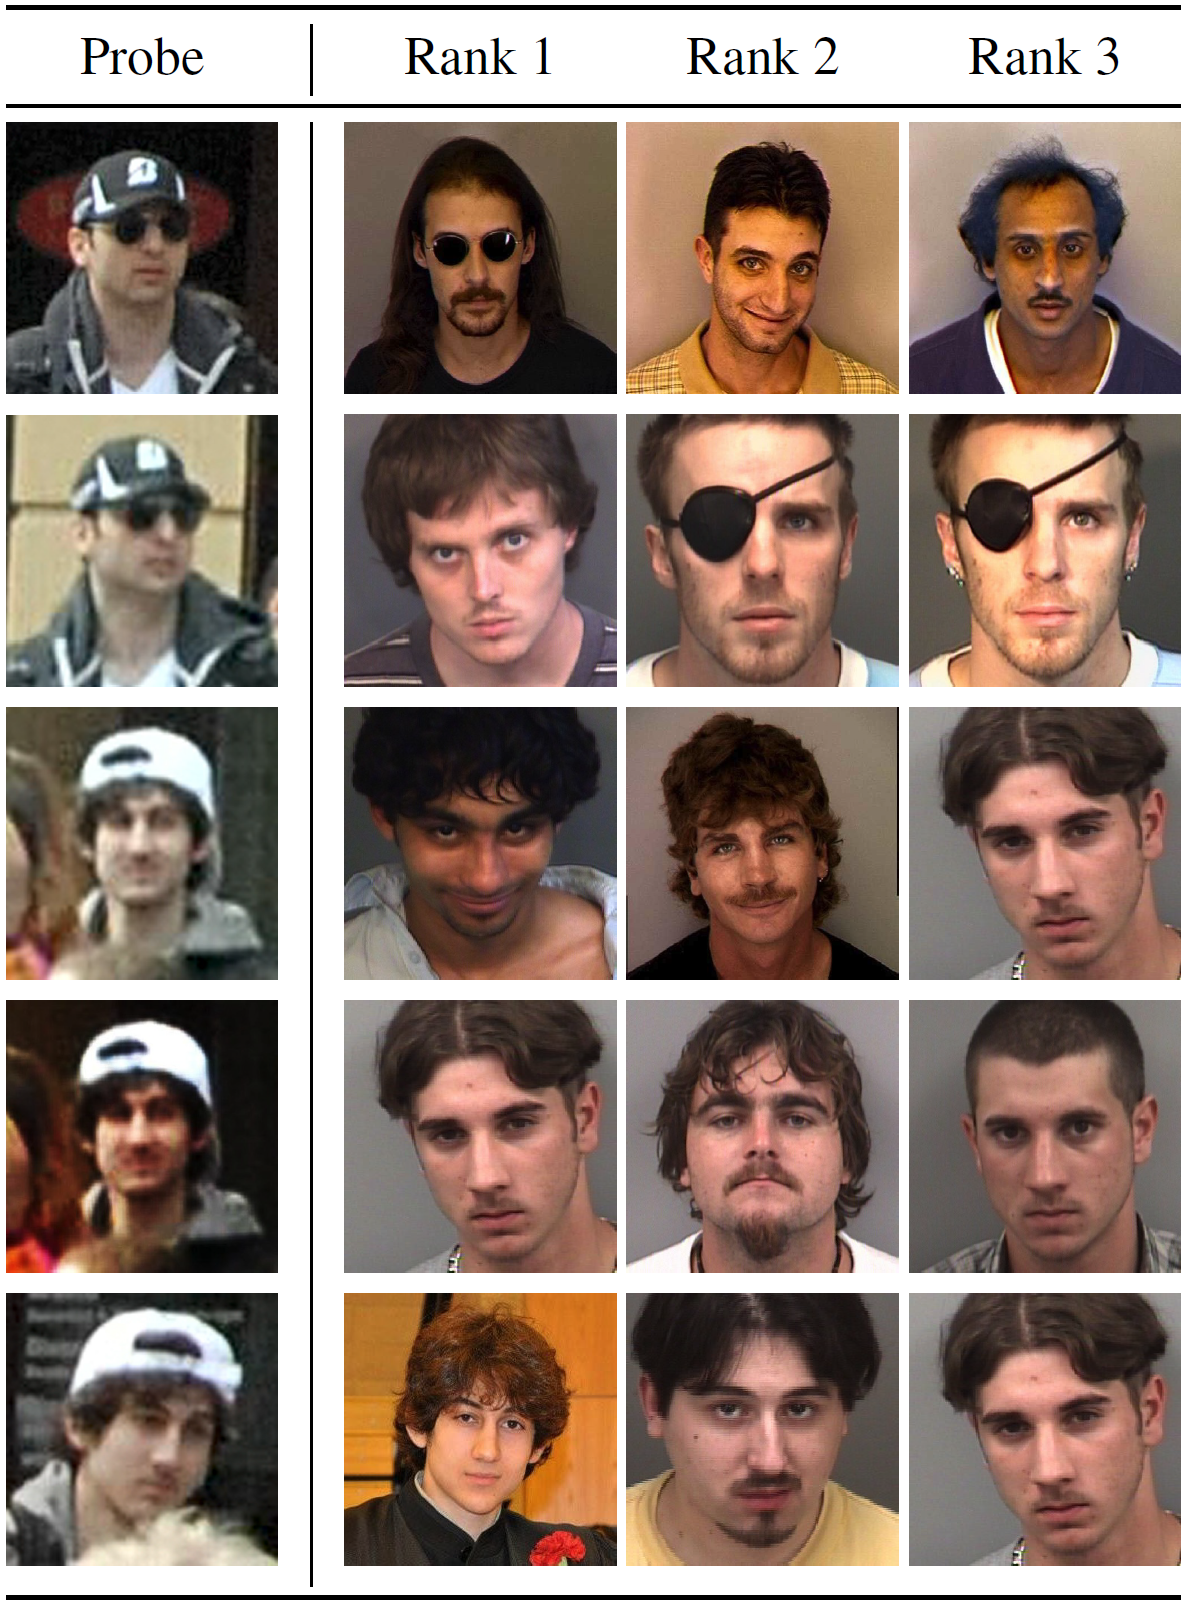
\includegraphics[scale=0.8]{res/boston_bomber.png}
Table of potential matches, note the correct identification from the picture taken from social media with similar pose and lighting \citep{bostonbombingcasestudy}.

\section{Connection Graph}
\label{appendix:connectiongraph}
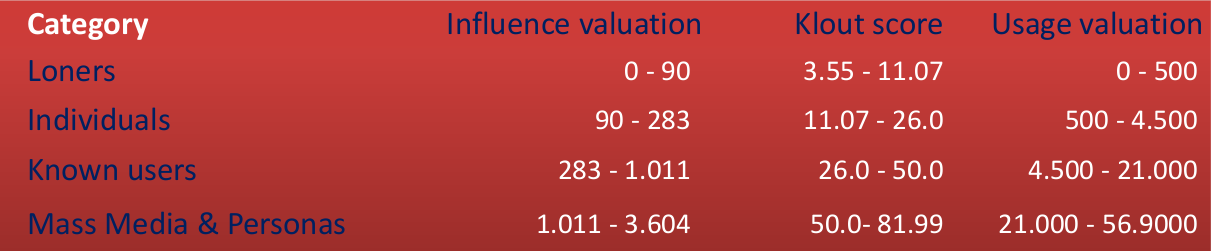
\includegraphics[width=\linewidth]{res/connection_klout.png}
Graph of social media connections and klout score in the Nereus framework\citep{behaviourdetection}.

\section{Command Line Arguments}
\label{appendix:commandlineargs}
\todo{Update with new image}
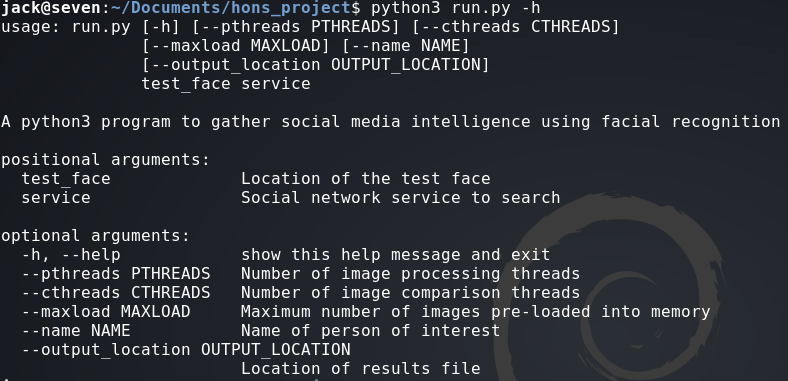
\includegraphics[width=\linewidth]{res/facegather_cmd_line_args.png}
A help page showing the command line arguments that can be supplied.

\end{appendices}
\end{document}